\documentclass[11pt]{article}
\usepackage{amsmath}
\usepackage{amssymb}
\usepackage{graphicx}
\usepackage{tabularx}
\usepackage{fancyhdr}
\usepackage{lastpage}

% Page layout
\usepackage[top=1in, bottom=1in, left=1in, right=1in]{geometry}

% Header and footer
\pagestyle{fancy}
\fancyhf{}
\rfoot{Page \thepage}
\renewcommand{\headrulewidth}{0pt}

% Modified Question command with left-aligned number
\newcommand{\questiona}[2]{
    \noindent\textbf{Q#2.} #1 \hfill \textbf{[1 Mark]}
}

\newcommand{\questionb}[2]{
    \noindent\textbf{Q#2.} #1 \hfill \textbf{[2 Marks]}
}

\begin{document}

% Title section with horizontal line
\begin{center}
    \Large\textbf{GATE 2017 - Mechanical Engineering (ME)} \\
    \large\textbf{General Aptitude and Technical Questions} \\
    \rule{\textwidth}{0.5pt} % Horizontal line below heading
\end{center}

\vspace{0.5cm}

% General Aptitude Section
\section*{General Aptitude}

\questiona{He was one of my best \_\_\_\_\_ and I felt his loss \_\_\_\_\_.}{1}
\begin{enumerate}
    \item[(A)] friend, keenly  
    \item[(B)] friends, keen  
    \item[(C)] friend, keener  
    \item[(D)] friends, keenly  
\end{enumerate}
\vspace{0.5cm}

\questiona{As the two speakers became increasingly agitated, the debate became \_\_\_\_\_.}{2}
\begin{enumerate}
    \item[(A)] lukewarm  
    \item[(B)] poetic  
    \item[(C)] forgiving  
    \item[(D)] heated  
\end{enumerate}
\vspace{0.5cm}

\questiona{A right-angled cone (with base radius 5 cm and height 12 cm), as shown in the figure below, is rolled on the ground keeping the point P fixed until the point Q (at the base of the cone, as shown) touches the ground again.}{3}
\begin{center}
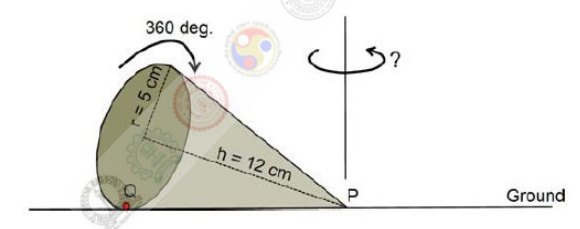
\includegraphics[width=0.5\textwidth]{figures/3.png}
\end{center}
By what angle (in radians) about P does the cone travel?
\begin{enumerate}
    \item[(A)] $\frac{5\pi}{12}$  
    \item[(B)] $\frac{5\pi}{24}$  
    \item[(C)] $\frac{24\pi}{5}$  
    \item[(D)] $\frac{10\pi}{13}$  
\end{enumerate}
\vspace{0.5cm}

\questiona{In a company with 100 employees, 45 earn Rs. 20,000 per month, 25 earn Rs. 30,000, 20 earn Rs. 40,000, 8 earn Rs. 60,000, and 2 earn Rs. 150,000. The median of the salaries is}{4}
\begin{enumerate}
    \item[(A)] Rs. 20,000  
    \item[(B)] Rs. 30,000  
    \item[(C)] Rs. 32,300  
    \item[(D)] Rs. 40,000  
\end{enumerate}
\vspace{0.5cm}

\questiona{P, Q, and R talk about S's car collection. P states that S has at least 3 cars. Q believes that S has less than 3 cars. R indicates that to his knowledge, S has at least one car. Only one of P, Q and R is right. The number of cars owned by S is}{5}
\begin{enumerate}
    \item[(A)] 0  
    \item[(B)] 1  
    \item[(C)] 3  
    \item[(D)] Cannot be determined  
\end{enumerate}
\vspace{0.5cm}

\questionb{"Here, throughout the early 1820s, Stuart continued to fight his losing battle to allow his sepoys to wear their caste-marks and their own choice of facial hair on parade, being again reprimanded by the commander-in-chief. His retort that 'A stronger instance than this of European prejudice with relation to this country has never come under my observations' had no effect on his superiors."}{6}

According to this paragraph, which of the statements below is most accurate?
\begin{enumerate}
    \item[(A)] Stuart's commander-in-chief was moved by this demonstration of his prejudice.  
    \item[(B)] The Europeans were accommodating of the sepoys' desire to wear their caste-marks.  
    \item[(C)] Stuart's 'losing battle' refers to his inability to succeed in enabling sepoys to wear caste-marks.  
    \item[(D)] The commander-in-chief was exempt from the European prejudice that dictated how the sepoys were to dress.  
\end{enumerate}
\vspace{0.5cm}

\questionb{What is the sum of the missing digits in the subtraction problem below?}{7}
\[
\frac{5\_\_\_}{-48\_} = 89
\]
\begin{enumerate}
    \item[(A)] 8  
    \item[(B)] 10  
    \item[(C)] 11  
    \item[(D)] Cannot be determined  
\end{enumerate}
\vspace{0.5cm}

\questionb{Let S$_1$ be the plane figure consisting of the points $(x, y)$ given by the inequalities $|x - 1| \leq 2$ and $|y + 2| \leq 3$. Let S$_2$ be the plane figure given by the inequalities $x - y \geq -2$, $y \geq 1$, and $x \leq 3$. Let S be the union of S$_1$ and S$_2$. The area of S is}{8}
\begin{enumerate}
    \item[(A)] 26  
    \item[(B)] 28  
    \item[(C)] 32  
    \item[(D)] 34  
\end{enumerate}
\vspace{0.5cm}

\questionb{Two very famous sportsmen Mark and Steve happened to be brothers, and played for country K. Mark teased James, an opponent from country E, "There is no way you are good enough to play for your country." James replied, "Maybe not, but at least I am the best player in my own family."\\ 
Which one of the following can be inferred from this conversation?}{9}
\begin{enumerate}
    \item [(A)] Mark was known to play better than James
    \item[(B)] Steve was known to play better than Mark
    \item[(C)] James and Steve were good friends
    \item[(D)] James played better than Steve 
\end{enumerate}
\vspace{0.5cm}

\questionb{The growth of bacteria \(lactobacillus\) in milk leads to curd formation. A minimum bacterial population density of 0.8 \(in suitable units\) is needed to form curd. In the graph below, the population density of lactobacillus in 1 litre of milk is plotted as a function of time, at two different temperatures, 25 C and 37 C.
\begin{center}
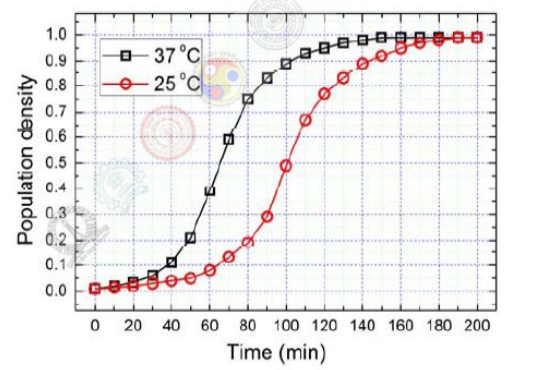
\includegraphics[width=0.5\textwidth]{figures/10.png}
\end{center}
Consider the following statements based on the data shown above: \\
i. The growth in bacterial population stops earlier at 37 C as compared to 25 C \\
ii. The time taken for curd formation at 25 C is twice the time taken at 37 C \\
Which one of the following options are correct?
}{10}
\begin{enumerate}
    \item [(A)] Only i
    \item[(B)] Only ii
    \item[(C)] Both i and II
    \item[(D)] Neither i nor ii
\end{enumerate}
\vspace{0.5cm}

% Technical Section
\section*{Technical Section}

\questiona{The product of eigenvalues of the matrix \( P \) is  
\[P = \begin{bmatrix} 
2 & 0 & 1 \\ 
4 & -3 & 3 \\ 
0 & 2 & -1 
\end{bmatrix}\]}{1}
\begin{enumerate}
    \item[(A)] \(-6\)  
    \item[(B)] 2  
    \item[(C)] 6  
    \item[(D)] \(-2\)
\end{enumerate}
\vspace{0.5cm}

\questiona{The value of \(\lim_{x \to 0} \frac{x^3 - \sin(x)}{x}\) is}{2}
\begin{enumerate}
    \item[(A)] 0  
    \item[(B)] 3  
    \item[(C)] 1  
    \item[(D)] \(-1\)
\end{enumerate}
\vspace{0.5cm}

\questiona{Consider the following partial differential equation for \( u(x, y) \) with the constant \( c > 1 \):  
\[\frac{\partial u}{\partial y} + c \frac{\partial u}{\partial x} = 0\]  
Solution of this equation is}{3}
\begin{enumerate}
    \item[(A)] \( u(x, y) = f(x + cy) \)  
    \item[(B)] \( u(x, y) = f(x - cy) \)  
    \item[(C)] \( u(x, y) = f(cx + y) \)  
    \item[(D)] \( u(x, y) = f(cx - y) \)
\end{enumerate}
\vspace{0.5cm}

\questiona{The differential equation \(\left. \frac{d^2y}{dx^2} \right|_{x=0} = 1\) and \(\left. \frac{dy}{dx} \right|_{x=\frac{\pi}{2}} = -1\) has}{4}
\begin{enumerate}
    \item[(A)] no solution  
    \item[(B)] exactly two solutions  
    \item[(C)] exactly one solution  
    \item[(D)] infinitely many solutions
\end{enumerate}
\vspace{0.5cm}

\questiona{A six-face fair dice is rolled a large number of times. The mean value of the outcomes is \_\_\_\_\_.}{5}
\vspace{0.5cm}

\questiona{For steady flow of a viscous incompressible fluid through a circular pipe of constant diameter, the average velocity in the fully developed region is constant. Which one of the following statements about the average velocity in the developing region is TRUE?}{6}
\begin{enumerate}
    \item[(A)] It increases until the flow is fully developed.
    \item[(B)] It is constant and is equal to the average velocity in the fully developed region.
    \item[(C)] It decreases until the flow is fully developed.
    \item[(D)] It is constant but is always lower than the average velocity in the fully developed region.
\end{enumerate}
\vspace{0.5cm}

\questiona{Consider the two-dimensional velocity field given by \( \vec{V} = (5 + a_1 x + b_1 y)i + (4 + a_2 x + b_2 y)j \), where \( a_1, b_1, a_2 \) and \( b_2 \) are constants. Which one of the following conditions needs to be satisfied for the flow to be incompressible?}{7}
\begin{enumerate}
    \item[(A)] \( a_1 + b_1 = 0 \)
    \item[(B)] \( a_1 + b_2 = 0 \)
    \item[(C)] \( a_2 + b_2 = 0 \)
    \item[(D)] \( a_2 + b_1 = 0 \)
\end{enumerate}
\vspace{0.5cm}

\questiona{Water (density = 1000 kg/m\(^3\)) at ambient temperature flows through a horizontal pipe of uniform cross section at the rate of 1 kg/s. If the pressure drop across the pipe is 100 kPa, the minimum power required to pump the water across the pipe, in watts, is \_\_\_\_\_.}{8}
\vspace{0.5cm}

\questiona{Which one of the following is NOT a rotating machine?}{9}
\begin{enumerate}
    \item[(A)] Centrifugal pump
    \item[(B)] Gear pump
    \item[(C)] Jet pump
    \item[(D)] Vane pump
\end{enumerate}
\vspace{0.5cm}

\questiona{Saturated steam at \( 100^\circ C \) condenses on the outside of a tube. Cold fluid enters the tube at \( 20^\circ C \) and exits at \( 50^\circ C \). The value of the Log Mean Temperature Difference (LMTD) is \_\_\_\_\_°C.}{10}
\vspace{0.5cm}

\questiona{The molar specific heat at constant volume of an ideal gas is equal to 2.5 times the universal gas constant (8.314 J/mol·K). When the temperature increases by 100 K, the change in molar specific enthalpy is \_\_\_\_\_ J/mol.}{11}
\vspace{0.5cm}

\questiona{A heat pump absorbs 10 kW of heat from outside environment at 250 K while absorbing 15 kW of work. It delivers the heat to a room that must be kept warm at 300 K. The Coefficient of Performance (COP) of the heat pump is \_\_\_\_\_.}{12}
\vspace{0.5cm}

\questiona{The Poisson's ratio for a perfectly incompressible linear elastic material is}{13}
\begin{enumerate}
    \item[(A)] 1  
    \item[(B)] 0.5  
    \item[(C)] 0  
    \item[(D)] infinity
\end{enumerate}
\vspace{0.5cm}

\questiona{A particle of unit mass is moving on a plane. Its trajectory, in polar coordinates, is given by  
\[ r(t) = t^2, \, \theta(t) = t, \]  
where \( t \) is time. The kinetic energy of the particle at time \( t = 2 \) is}{14}
\begin{enumerate}
    \item[(A)] 4  
    \item[(B)] 12  
    \item[(C)] 16  
    \item[(D)] 24
\end{enumerate}
\vspace{0.5cm}

\questiona{A motor driving a solid circular steel shaft transmits 40 kW of power at 500 rpm. If the diameter of the shaft is 40 mm, the maximum shear stress in the shaft is \_\_\_\_\_ MPa.}{15}
\vspace{0.5cm}

\questiona{Consider a beam with circular cross-section of diameter \( d \). The ratio of the second moment of area about the neutral axis to the section modulus of the area is}{16}
\begin{enumerate}
    \item[(A)] \(\frac{d}{2}\)  
    \item[(B)] \(\frac{\pi d}{2}\)  
    \item[(C)] \(d\)  
    \item[(D)] \(\pi d\)
\end{enumerate}
\vspace{0.5cm}

\questiona{The following figure shows the velocity-time plot for a particle traveling along a straight line. The distance covered by the particle from \( t = 0 \) to \( t = 5 \, \text{s} \) is \_\_\_\_\_ m.}{17}
\begin{center}
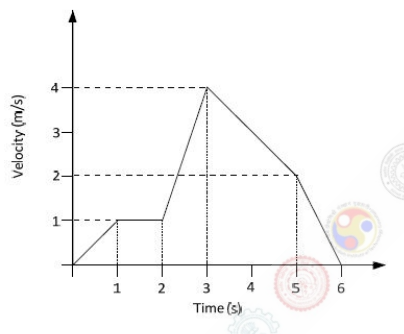
\includegraphics[width=0.5\textwidth]{figures/17.png}
\end{center}
\vspace{0.5cm}

\questiona{The damping ratio for a viscously damped spring mass system, governed by the relationship  
\[m \frac{d^2 x}{dt^2} + c \frac{dx}{dt} + kx = F(t),\]  
is given by}{18}
\begin{enumerate}
    \item[(A)] \(\sqrt{\frac{c}{mk}}\)  
    \item[(B)] \(\frac{c}{2\sqrt{km}}\)  
    \item[(C)] \(\frac{c}{\sqrt{km}}\)  
    \item[(D)] \(\sqrt{\frac{c}{2mk}}\)
\end{enumerate}
\vspace{0.5cm}

\questiona{Consider the schematic of a riveted lap joint subjected to tensile load \( F \), as shown below. Let \( d \) be the diameter of the rivets, and \( S_f \) be the maximum permissible tensile stress in the plates. What should be the minimum value for the thickness of the plates to guard against tensile failure of the plates? Assume the plates to be identical.}{19}
\begin{center}
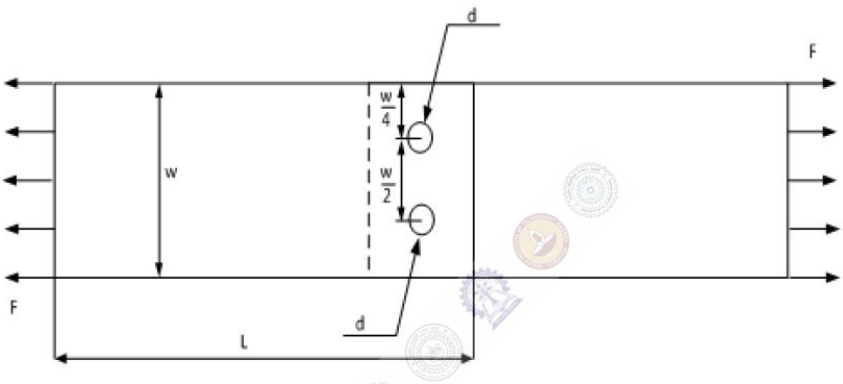
\includegraphics[width=0.8\textwidth]{figures/19.png}
\end{center}
\begin{enumerate}
    \item[(A)] \( \frac{F}{S_f (W - 2d)} \)  
    \item[(B)] \( \frac{F}{S_f W} \)  
    \item[(C)] \( \frac{F}{S_f (W - d)} \)  
    \item[(D)] \( \frac{2F}{S_f W} \)
\end{enumerate}
\vspace{0.5cm}

\questiona{Cylindrical pins of diameter \( 15^{\pm 0.020} \) mm are being produced on a machine. Statistical quality control tests show a mean of 14.995 mm and standard deviation of 0.004 mm. The process capability index \( Cp \) is}{20}
\begin{enumerate}
    \item[(A)] 0.833  
    \item[(B)] 1.667  
    \item[(C)] 3.333  
    \item[(D)] 3.750
\end{enumerate}
\vspace{0.5cm}

\questiona{In a metal forming operation when the material has just started yielding, the principal stresses are \( \sigma_1 = +180 \, \text{MPa}, \, \sigma_2 = -100 \, \text{MPa}, \, \sigma_3 = 0 \). Following von Mises' criterion, the yield stress is \_\_\_\_\_ MPa.}{21}
\vspace{0.5cm}

\questiona{Match the processes with their characteristics.}{22}
\begin{center}
\begin{tabular}{|l|l|}
\hline
Process & Characteristics \\
\hline
P: Electrical Discharge Machining & 1. No residual stress \\
Q: Ultrasonic machining & 2. Machining of electrically conductive materials \\
R: Chemical machining & 3. Machining of glass \\
S: Ion Beam Machining & 4. Nano-machining \\
\hline
\end{tabular}
\end{center}
\begin{enumerate}
    \item[(A)] P-2, Q-3, R-1, S-4  
    \item[(B)] P-3, Q-2, R-1, S-4  
    \item[(C)] P-3, Q-2, R-4, S-1  
    \item[(D)] P-2, Q-4, R-3, S-1
\end{enumerate}
\vspace{0.5cm}

\questiona{In an arc welding process, welding speed is doubled. Assuming all other process parameters to be constant, the cross sectional area of the weld bead will}{23}
\begin{enumerate}
    \item[(A)] increase by 25 \%  
    \item[(B)] increase by 50 \%  
    \item[(C)] reduce by 25 \%  
    \item[(D)] reduce by 50 \%
\end{enumerate}
\vspace{0.5cm}

\questiona{Metric thread of 0.8 mm pitch is to be cut on a lathe. Pitch of the lead screw is 1.5 mm. If the spindle rotates at 1500 rpm, the speed of rotation of the lead screw (rpm) will be \_\_\_\_\_.}{24}
\vspace{0.5cm}

\questiona{In the engineering stress-strain curve for mild steel, the Ultimate Tensile Strength (UTS) refers to}{25}
\begin{enumerate}
    \item[(A)] Yield stress  
    \item[(B)] Proportional limit  
    \item[(C)] Maximum stress  
    \item[(D)] Fracture stress
\end{enumerate}
\vspace{0.5cm}

\questionb{Consider the matrix \( P = \begin{bmatrix} \frac{1}{\sqrt{2}} & 0 & \frac{1}{\sqrt{2}} \\ 0 & 1 & 0 \\ -\frac{1}{\sqrt{2}} & 0 & \frac{1}{\sqrt{2}} \end{bmatrix} \). Which one of the following statements about \( P \) is INCORRECT?}{26}
\begin{enumerate}
    \item[(A)] Determinant of \( P \) is equal to 1.
    \item[(B)] \( P \) is orthogonal.
    \item[(C)] Inverse of \( P \) is equal to its transpose.
    \item[(D)] All eigenvalues of \( P \) are real numbers.
\end{enumerate}
\vspace{0.5cm}

\questionb{For the vector \( \vec{V} = 2yz \hat{i} + 3xz \hat{j} + 4xy \hat{k} \), the value of \( \nabla. (\nabla \times \vec{V}) \) is \_\_\_\_\_.}{27}
\vspace{0.5cm}

\questionb{A parametric curve defined by \( x = \cos \left( \frac{\pi u}{2} \right), y = \sin \left( \frac{\pi u}{2} \right) \) in the range \( 0 \leq u \leq 1 \) is rotated about the X-axis by 360 degrees. Area of the surface generated is}{28}
\begin{enumerate}
    \item[(A)] \( \frac{\pi}{2} \)
    \item[(B)] \( \pi \)
    \item[(C)] \( 2\pi \)
    \item[(D)] \( 4\pi \)
\end{enumerate}
\vspace{0.5cm}

\questionb{\( P (0, 3), Q (0.5, 4), \) and \( R (1, 5) \) are three points on the curve defined by \( f(x) \). Numerical integration is carried out using both Trapezoidal rule and Simpson's rule within limits \( x = 0 \) and \( x = 1 \) for the curve. The difference between the two results will be}{29}
\begin{enumerate}
    \item[(A)] 0
    \item[(B)] 0.25
    \item[(C)] 0.5
    \item[(D)] 1
\end{enumerate}
\vspace{0.5cm}

\questionb{The velocity profile inside the boundary layer for flow over a flat plate is given as \(\frac{u}{U_{\infty}} = \sin \left( \frac{\pi y}{2 \delta} \right)\), where \( U_{\infty} \) is the free stream velocity and \(\delta\) is the local boundary layer thickness. If \(\delta^*\) is the local displacement thickness, the value of \(\frac{\delta^*}{\delta}\) is}{30}
\begin{enumerate}
    \item[(A)] \(\frac{2}{\pi}\)
    \item[(B)] \(1 - \frac{2}{\pi}\)
    \item[(C)] \(1 + \frac{2}{\pi}\)
    \item[(D)] 0
\end{enumerate}
\vspace{0.5cm}

\questionb{Consider steady flow of an incompressible fluid through two long and straight pipes of diameters \( d_1 \) and \( d_2 \) arranged in series. Both pipes are of equal length and the flow is turbulent in both pipes. The friction factor for turbulent flow though pipes is of the form, \( f = K(\text{Re})^{-n} \), where \( K \) and \( n \) are known positive constants and Re is the Reynolds number. Neglecting minor losses, the ratio of the frictional pressure drop in pipe 1 to that in pipe 2, \(\left( \frac{\Delta P_1}{\Delta P_2} \right)\), is given by}{31}
\begin{enumerate}
    \item[(A)] \(\left( \frac{d_2}{d_1} \right)^{(5-n)}\)
    \item[(B)] \(\left( \frac{d_2}{d_1} \right)^5\)
    \item[(C)] \(\left( \frac{d_2}{d_1} \right)^{(3-n)}\)
    \item[(D)] \(\left( \frac{d_2}{d_1} \right)^{(5+n)}\)
\end{enumerate}
\vspace{0.5cm}

\questionb{For a steady flow, the velocity field is \(\vec{V} = (-x^2 + 3y) \hat{i} + (2xy) \hat{j}\). The magnitude of the acceleration of a particle at \((1, -1)\) is}{32}
\begin{enumerate}
    \item[(A)] 2
    \item[(B)] 1
    \item[(C)] \(2\sqrt{5}\)
    \item[(D)] 0
\end{enumerate}
\vspace{0.5cm}

\questionb{One kg of an ideal gas (gas constant, \( R = 400 \, \text{J/kg} \). K ; specific heat at constant volume, \( c_v = 1000 \, \text{J/kg} \). K) at 1 bar, and 300 K is contained in a sealed rigid cylinder. During an adiabatic process, 100 kJ of work is done on the system by a stirrer. The increase in entropy of the system is \_\_\_\_\_ J/K.}{33}
\vspace{0.5cm}

\questionb{The pressure ratio across a gas turbine (for air, specific heat at constant pressure, \( c_p = 1040 \, \text{J/kg} \). K and ratio of specific heats, \( \gamma = 1.4 \)) is 10. If the inlet temperature to the turbine is 1200 K and the isentropic efficiency is 0.9, the gas temperature at turbine exit is \_\_\_\_\_ K.}{34}
\vspace{0.5cm}

\questionb{Moist air is treated as an ideal gas mixture of water vapor and dry air (molecular weight of air = 28.84 and molecular weight of water = 18). At a location, the total pressure is 100 kPa, the temperature is 30 °C and the relative humidity is 55\%. Given that the saturation pressure of water at 30 °C is 4246 Pa, the mass of water vapor per kg of dry air is \_\_\_\_\_ grams.}{35}
\vspace{0.5cm}

\questionb{Air contains 79\% \( \text{N}_2 \) and 21\% \( \text{O}_2 \) on a molar basis. Methane (CH\(_4\)) is burned with 50\% excess air than required stoichiometrically. Assuming complete combustion of methane, the molar percentage of \( \text{N}_2 \) in the products is \_\_\_\_\_.}{36}
\vspace{0.5cm}

\questionb{Two black surfaces, AB and BC, of lengths 5 m and 6 m, respectively, are oriented as shown. Both surfaces extend infinitely into the third dimension. Given that view factor \( F_{12} = 0.5, T_1 = 800\text{K}, T_2 = 600\text{K}, T_{\text{surrounding}} = 300\text{K} \) and Stefan Boltzmann constant, \( \sigma = 5.67 \times 10^{-8}\text{W}/(\text{m}^2\text{K}^4) \), the heat transfer rate from Surface 2 to the surrounding environment is \_\_\_\_\_ kW.}{37}
\begin{center}
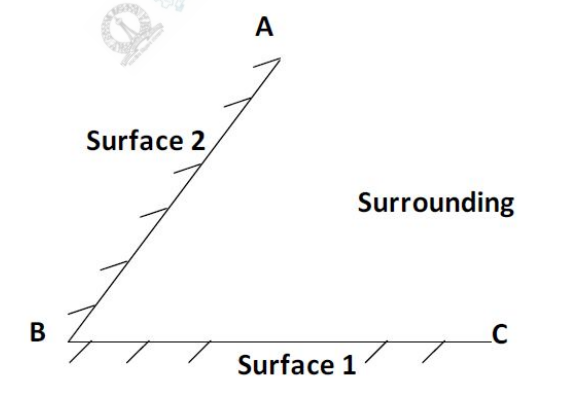
\includegraphics[width=0.5\textwidth]{figures/37.png}
\end{center}
\vspace{0.5cm}

\questionb{Heat is generated uniformly in a long solid cylindrical rod (diameter = 10 mm) at the rate of \( 4 \times 10^7 \, \text{W/m}^3 \). The thermal conductivity of the rod material is 25 W/m.K. Under steady state conditions, the temperature difference between the centre and the surface of the rod is \_\_\_\_\_°C.}{38}
\vspace{0.5cm}

\questionb{An initially stress-free massless elastic beam of length \( L \) and circular cross-section with diameter \( d \) (\( d < L \)) is held fixed between two walls as shown. The beam material has Young's modulus \( E \) and coefficient of thermal expansion \( \alpha \). If the beam is slowly and uniformly heated, the temperature rise required to cause the beam to buckle is proportional to}{39}
\begin{center}
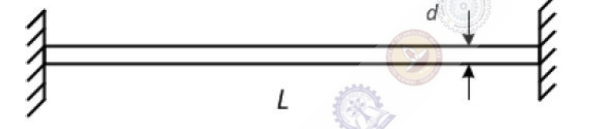
\includegraphics[width=0.7\textwidth]{figures/39.png}
\end{center}
\begin{enumerate}
    \item[(A)] \( d \)
    \item[(B)] \( d^2 \)
    \item[(C)] \( d^3 \)
    \item[(D)] \( d^4 \)
\end{enumerate}
\vspace{0.5cm}

\questionb{A point mass of 100 kg is dropped onto a massless elastic bar (cross-sectional area = 100 mm\(^2\), length = 1 m, Young's modulus = 100 GPa) from a height \( H \) of 10 mm as shown (Figure is not to scale). If \( g = 10 \, \text{m/s}^2 \), the maximum compression of the elastic bar is \_\_\_\_\_ mm.}{40}
\begin{center}
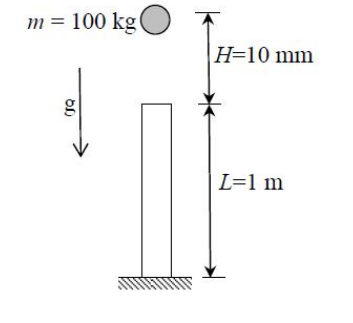
\includegraphics[width=0.5\textwidth]{figures/40.png}
\end{center}
\vspace{0.5cm}

\questionb{Two disks A and B with identical mass (\(m\)) and radius (\(R\)) are initially at rest. They roll down from the top of identical inclined planes without slipping. Disk A has all of its mass concentrated at the rim, while Disk B has its mass uniformly distributed. At the bottom of the plane, the ratio of velocity of the center of disk A to the velocity of the center of disk B is}{41}
\begin{enumerate}
    \item[(A)] \(\sqrt{\frac{3}{4}}\)
    \item[(B)] \(\sqrt{\frac{3}{2}}\)
    \item[(C)] 1
    \item[(D)] \(\sqrt{2}\)
\end{enumerate}
\vspace{0.5cm}

\questionb{A rectangular region in a solid is in a state of plane strain. The (\(x,y\)) coordinates of the corners of the undeformed rectangle are given by \(P(0,0)\), \(Q(4,0)\), \(R(4,3)\), \(S(0,3)\). The rectangle is subjected to uniform strains, \(\varepsilon_{xx} = 0.001\), \(\varepsilon_{yy} = 0.002\), \(\gamma_{xy} = 0.003\). The deformed length of the elongated diagonal, upto three decimal places, is \_\_\_\_\_ units.}{42}
\vspace{0.5cm}

\questionb{A machine element has an ultimate strength (\(\sigma_u\)) of 600 N/mm\(^2\), and endurance limit (\(\sigma_{en}\)) of 250 N/mm\(^2\). The fatigue curve for the element on a \textbf{log-log} plot is shown below. If the element is to be designed for a finite life of 10000 cycles, the maximum amplitude of a completely reversed operating stress is \_\_\_\_\_ N/mm\(^2\).}{43}
\begin{center}
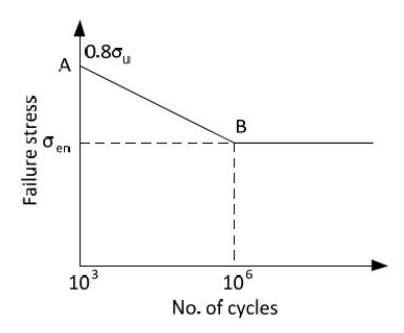
\includegraphics[width=0.5\textwidth]{figures/43.png}
\end{center}
\vspace{0.5cm}

\questionb{A horizontal bar, fixed at one end (\( x = 0 \)), has a length of 1 m, and cross-sectional area of 100 mm\(^2\). Its elastic modulus varies along its length as given by \( E(x) = 100 \, e^{-x} \, \text{GPa} \), where \( x \) is the length coordinate (in m) along the axis of the bar. An axial tensile load of 10 kN is applied at the free end (\( x = 1 \)). The axial displacement of the free end is \_\_\_\_\_ mm.}{44}
\vspace{0.5cm}

\questionb{In an epicyclic gear train, shown in the figure, the outer ring gear is fixed, while the sun gear rotates counterclockwise at 100 rpm. Let the number of teeth on the sun, planet and outer gears to be 50, 25, and 100, respectively. The ratio of magnitudes of angular velocity of the planet gear to the angular velocity of the carrier arm is \_\_\_\_\_.}{45}
\begin{center}
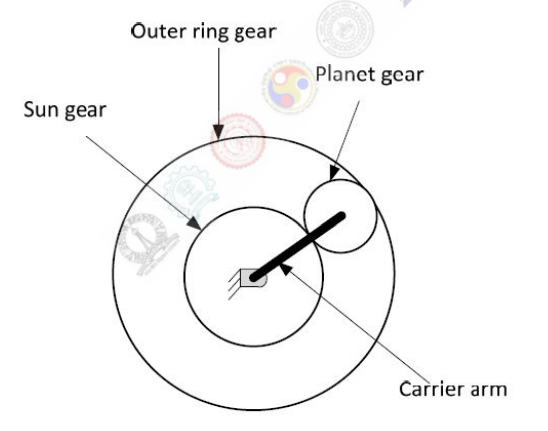
\includegraphics[width=0.5\textwidth]{figures/45.png}
\end{center}
\vspace{0.5cm}

\questionb{A thin uniform rigid bar of length \( L \) and mass \( M \) is hinged at point \( O \), located at a distance of \(\frac{L}{3}\) from one of its ends. The bar is further supported using springs, each of stiffness \( k \), located at the two ends. A particle of mass \( m = \frac{M}{4} \) is fixed at one end of the bar, as shown in the figure. For small rotations of the bar about \( O \), the natural frequency of the system is}{46}
\begin{center}
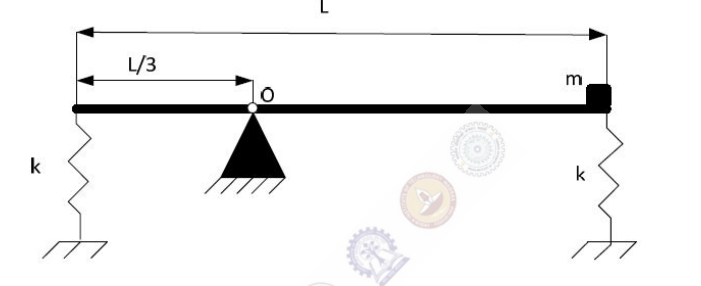
\includegraphics[width=0.7\textwidth]{figures/46.png}
\end{center}
\vspace{0.5cm}

\questionb{For an inline slider-crank mechanism, the lengths of the crank and connecting rod are 3 m and 4 m, respectively. At the instant when the connecting rod is perpendicular to the crank, if the velocity of the slider is 1 m/s, the magnitude of angular velocity (upto 3 decimal points accuracy) of the crank is \_\_\_\_\_ radian/s.}{47}
\vspace{0.5cm}

\questionb{A 10 mm deep cylindrical cup with diameter of 15 mm is drawn from a circular blank. Neglecting the variation in the sheet thickness, the diameter (upto 2 decimal points accuracy) of the blank is \_\_\_\_\_ mm.}{48}
\vspace{0.5cm}

\questionb{Circular arc on a part profile is being machined on a vertical CNC milling machine. CNC part program using metric units with absolute dimensions is listed below:}{49}
\begin{verbatim}
N60 G01 X 30 Y 55 Z -5 F50
N70 G02 X 50 Y 35 R 20
N80 G01 Z 5
\end{verbatim}
The coordinates of the centre of the circular arc are:
\begin{enumerate}
    \item[(A)] (30, 55)
    \item[(B)] (50, 55)
    \item[(C)] (50, 35)
    \item[(D)] (30, 35)
\end{enumerate}
\vspace{0.5cm}

\questionb{Assume that the surface roughness profile is triangular as shown schematically in the figure. If the peak to valley height is 20 \(\mu\)m, the central line average surface roughness \(R_a\) (in \(\mu\)m) is}{50}
\begin{center}
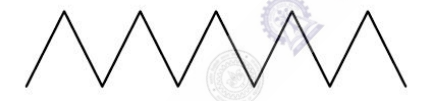
\includegraphics[width=0.5\textwidth]{figures/50.png}
\end{center}
\begin{enumerate}
    \item[(A)] 5
    \item[(B)] 6.67
    \item[(C)] 10
    \item[(D)] 20
\end{enumerate}
\vspace{0.5cm}

\questionb{Two models, P and Q, of a product earn profits of Rs. 100 and Rs. 80 per piece, respectively. Production times for P and Q are 5 hours and 3 hours, respectively, while the total production time available is 150 hours. For a total batch size of 40, to maximize profit, the number of units of P to be produced is \_\_\_\_\_.}{51}
\vspace{0.5cm}

\questionb{Following data refers to the jobs (P, Q, R, S) which have arrived at a machine for scheduling. The shortest possible average flow time is \_\_\_\_\_ days.}{52}
\begin{center}
\begin{tabular}{|l|l|}
\hline
Job & Processing Time (days) \\
\hline
P & 15 \\
Q & 9 \\
R & 22 \\
S & 12 \\
\hline
\end{tabular}
\end{center}
\vspace{0.5cm}

\questionb{A block of length 200 mm is machined by a slab milling cutter 34 mm in diameter. The depth of cut and table feed are set at 2 mm and 18 mm/minute, respectively. Considering the approach and the over travel of the cutter to be same, the minimum estimated machining time per pass is \_\_\_\_\_ minutes.}{53}
\vspace{0.5cm}

\questionb{A sprue in a sand mould has a top diameter of 20 mm and height of 200 mm. The velocity of the molten metal at the entry of the sprue is 0.5 m/s. Assume acceleration due to gravity as 9.8 m/s\(^2\) and neglect all losses. If the mould is well ventilated, the velocity (upto 3 decimal points accuracy) of the molten metal at the bottom of the sprue is \_\_\_\_\_ m/s.}{54}
\vspace{0.5cm}

\questionb{Two cutting tools with tool life equations given below are being compared:}{55}
\begin{center}
Tool 1: \( VT^{0.1} = 150 \) \\
Tool 2: \( VT^{0.3} = 300 \)
\end{center}
where \( V \) is cutting speed in m/minute and \( T \) is tool life in minutes. The breakeven cutting speed beyond which Tool 2 will have a higher tool life is \_\_\_\_\_ m/minute.
\vspace{0.5cm}

\vspace{5cm}
\begin{center}
\textbf{END OF THE QUESTION PAPER} \\
\rule{\textwidth}{0.5pt}
\end{center}

\end{document}
